\documentclass[a4paper,11pt]{article}

\usepackage[utf8]{inputenc}
\usepackage{minted}
\usepackage{pgfplots}
\pgfplotsset{compat=1.18}

\begin{document}

\title{
	\textbf{Towers of Hanoi - Report}
	}
\author{Adrian Hjert}
\date{09/Feb/2023}

\maketitle

\section*{
	\underline{Introduction}
}
The aim of this report is to shortly describe the implementation of some code in Elixir that solves the \textit{Towers of Hanoi} puzzle using a recursive strategy as well as provide answers to some questions regarding how the code behaves at different tower sizes.

\section*{
	\underline{Methods}
}
Much of the code is provided in the instruction sheet. The full code that solves the problem can be seen below, excluding the code for the test cases.

\begin{minted}{elixir}
 defmodule Hanoi do
 
def hanoi(0, _, _, _) do [] end
def hanoi(n, from, inter, to) do
  hanoi(n-1, from, to, inter) ++
  [{:move, from, to}] ++
  hanoi(n-1, inter, from, to)

end
end
\end{minted}

The first situation we can encounter is where we have no discs in the tower, where we return an empty list, since no moves are possible. This requires no recursion. The next situation we can encounter is when we have more than zero discs and wish to solve the puzzle. This can be done with a recursive strategy where, as the ''name'' suggests, the function \textit{hanoi/4} calls itself repeatedly until the problem is solved. It works in the following manner;
Initially, $n - 1$ discs are moved form the starting position to the intermediate, or middle, pillar. Each move is printed before the program continues with the recursion. We then move the discs to the finishing position, the \textit{to} pillar, printing these moves as well. The number of moves and the outputs for 1, 2, 3 and 4 discs were recorded. The output for 4 discs can be seen in the \textbf{Results and Conclusions} section of this report along with \textbf{Graph 1} showing the number of moves for each of these tower sizes. A formula to figure out how many moves are required for any tower size is derived using this data and will help us calculate and answer the question of how many moves are required for a tower size of 10.

\section*{
	\underline{Results and Conclusions}
}
The following shows the output of the code for 3 and 4 discs in the tower respectively.
\begin{minted}{elixir}
[
  {:move, :from, :to},
  {:move, :from, :inter},
  {:move, :to, :inter},
  {:move, :from, :to},
  {:move, :inter, :from},
  {:move, :inter, :to},
  {:move, :from, :to}
]
[
  {:move, :from, :inter},
  {:move, :from, :to},
  {:move, :inter, :to},
  {:move, :from, :inter},
  {:move, :to, :from},
  {:move, :to, :inter},
  {:move, :from, :inter},
  {:move, :from, :to},
  {:move, :inter, :to},
  {:move, :inter, :from},
  {:move, :to, :from},
  {:move, :inter, :to},
  {:move, :from, :inter},
  {:move, :from, :to},
  {:move, :inter, :to}
]
\end{minted}
as we can see, the number of moves grows rather quick between 3 and 4. \textbf{Graph 1} highlights this.

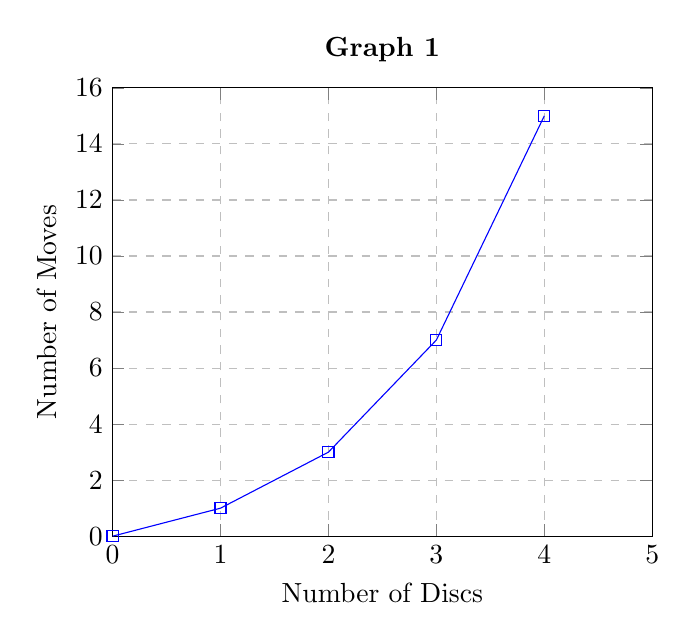
\begin{tikzpicture}
\begin{axis}[
	title = {\textbf{Graph 1}},
	xlabel ={Number of Discs},
	ylabel = {Number of Moves},
xmin = 0, xmax = 5,
ymin = 0, ymax = 16,
xtick = {0, 1, 2, 3, 4, 5},
ytick = {0, 2, 4, 6, 8, 10, 12, 14, 16},
ymajorgrids = true,
xmajorgrids = true,
grid style = dashed
]

\addplot[
color = blue,
mark = square,
]
coordinates{
(0, 0)(1, 1)(2, 3)(3, 7)(4, 15)
};

\end{axis}
\end{tikzpicture}

Using \textbf{Graph 1} we can determine that the number of moves follows the function $f(n) = 2^n - 1$ where $n$ is the number of discs and $f(n)$ gives the number of moves needed to solve the puzzle. To calculate the number of moves needed for a tower of size 10, so 10 discs, we simply do $f(10) = 2^{10} -1$ which is $1024 -1$ which is $1023$. So, to solve this puzzle with 10 discs, we need to perform 1023 moves.



\end{document}